\chapter{Onglet Profils}
\label{chap:profils}

L'onglet \menu{Profils} est le cœur de l'application : il permet
le chargement, la visualisation, l'édition et la comparaison des
profils. Au démarrage, le profil courant (bleu) est un
\textbf{NACA~2412} automatiquement \textbf{converti en Bézier}, et
le profil de référence (rouge) est un \textbf{NACA~2412} en mode
points discrets. Par défaut, la \textbf{courbure} du courant, la
\textbf{déviation} entre les deux profils et le \textbf{volet}
(braqué à $-10^\circ$) sont également affichés.

\screenshot{02_tab_profils_default.png}{1.0}{%
    Onglet \menu{Profils} dans son état par défaut : profil courant
    (bleu, Bézier) avec ses points de contrôle, courbure au bord
    d'attaque, profil avec volet (vert) et déviation par rapport à
    la référence.}

\section{Barre de contrôle}

La barre située sous le sélecteur d'onglets regroupe les options
d'affichage, organisées en \textbf{quatre cadres} selon qu'elles
concernent un seul profil, les deux, ou aucun.

\subsubsection*{Cadre \og Profil courant \fg{}}

\begin{itemize}
    \item \textbf{Profil courant} (case à cocher) : affiche ou
        masque le profil courant. L'étiquette colorée indique
        son nom (par défaut \og NACA~2412 \fg{}).
    \item \textbf{Courbure} : affiche les \emph{porcupines} de
        courbure du profil courant (segments perpendiculaires à la
        courbe, longueur proportionnelle à la courbure locale).
    \item \textbf{Pts} : affiche les points effectivement
        échantillonnés sur les splines (marqueurs).
\end{itemize}

\subsubsection*{Cadre \og Profil référence \fg{}}

\begin{itemize}
    \item \textbf{Profil référence} et \textbf{Courbure} :
        idem pour le profil de référence.
\end{itemize}

\subsubsection*{Cadre global (deux profils / aucun)}

\begin{itemize}
    \item \textbf{Déviation} : trace les écarts géométriques
        entre profil courant et référence. Le \textbf{mode} de calcul
        (verticale ou normale) se choisit dans le menu
        \menu{Options $\rightarrow$ Déviation}. Voir
        section~\ref{sec:deviation}, page~\pageref{sec:deviation}.
    \item \textbf{Image} : affiche ou masque l'\textbf{image de
        calque} (arrière-plan) lorsqu'une image a été chargée.
        La case reste inactive (grisée) tant qu'aucune image n'est
        chargée. Voir la section~\ref{sec:calque},
        page~\pageref{sec:calque}.
\end{itemize}

\subsubsection*{Cadre \og Flap \fg{} (volet)}

\begin{itemize}
    \item \textbf{Flap} (case à cocher) : active la génération et
        l'affichage d'un profil avec volet braqué (vert).
    \item \textbf{Xf} : position de l'axe d'articulation, en pourcent
        de corde depuis le bord d'attaque.
    \item \textbf{Braquage} : angle de braquage du volet, en degrés
        (positif = bord de fuite vers le haut).
\end{itemize}

Le module de volet est détaillé en section~\ref{sec:flap},
page~\pageref{sec:flap}.

\begin{important}
Les options \textbf{Courbure} ne fonctionnent que sur des
profils en \textbf{mode spline}. Si vous tentez de les activer
sur un profil en mode points discrets, un message
d'avertissement s'affiche et la case se décoche
automatiquement (voir \figref{08_msg_courbure.png}).
\end{important}

\section{Visualisation des profils}

\subsection{Mode points discrets}

C'est le mode par défaut au chargement. Le profil est tracé sous
forme de courbe lisse interpolée entre les points discrets. Aucun
point de contrôle n'est visible.

\subsection{Mode spline}

Une fois le profil converti en spline (voir
section~\ref{sec:convertspline}), de nombreux éléments
apparaissent :

\screenshot{03_tab_profils_spline.png}{1.0}{%
    Profil en mode spline : les carrés bleus sont les points
    de contrôle intérieurs des Béziers ; les points entourés
    d'un cercle marquent les jonctions entre segments
    consécutifs.}

\begin{itemize}
    \item \textbf{Carrés bleus} : points de contrôle intérieurs
        des courbes de Bézier. Ils sont \textbf{déplaçables}
        à la souris pour modifier la forme du profil.
    \item \textbf{Cercles avec point central} : points de jonction
        entre deux segments de Bézier consécutifs. Ils sont
        également déplaçables ; leur déplacement préserve la
        continuité C\textsuperscript{1} avec les segments voisins.
    \item \textbf{Polygone de contrôle} (lignes pointillées
        grises) : relie les points de contrôle dans l'ordre.
    \item \textbf{Ligne moyenne} (pointillé bleu clair) :
        trace la cambrure relative du profil (moyenne
        extrados/intrados).
\end{itemize}

\subsection{Affichage de la courbure}

L'activation de la case \textbf{Courbure} fait apparaître les
\emph{porcupines} : segments perpendiculaires à la courbe, dont
la longueur est proportionnelle à la courbure locale signée.

\screenshot{04_tab_profils_courbure.png}{1.0}{%
    Affichage des porcupines de courbure (segments oranges).}

\begin{noteinfo}
La courbure est l'inverse du rayon du cercle osculateur.
Une courbure positive signale une courbe concave vers les
$y$ croissants (sommet de l'extrados), négative concave vers
les $y$ décroissants. Les discontinuités de courbure sont
souvent visibles aux jonctions de segments en continuité C1
mais non C2.
\end{noteinfo}

L'\textbf{échelle des porcupines} et leur \textbf{densité}
(nombre de quills par courbe) sont réglables via le menu
contextuel (clic droit sur le canvas).

\subsection{Affichage des points échantillonnés}

L'option \textbf{Pts} fait apparaître des marqueurs aux positions
des points effectivement utilisés pour l'échantillonnage
discret. C'est utile pour vérifier la densité et la répartition
de l'échantillonnage avant export ou simulation.

\screenshot{05_tab_profils_pts.png}{1.0}{%
    Affichage des points d'échantillonnage. Le mode
    \emph{curviligne} (par défaut) répartit les points
    de manière uniforme le long de l'arc.}

\subsection{Visualisation de la déviation}
\label{sec:deviation}

L'option \textbf{Déviation} mesure l'écart géométrique entre le
profil courant et le profil de référence, sous forme d'un faisceau
de segments (\emph{quills}) accompagné d'une enveloppe. Le maximum
de déviation est mis en évidence.

\subsubsection*{Modes de calcul}

Le mode se choisit dans le menu \menu{Options $\rightarrow$
Déviation} :

\begin{itemize}
    \item \textbf{Verticale (épaisseur)} : l'écart est mesuré
        \textbf{verticalement} (selon l'axe $z$), à abscisse $x$
        constante, par interpolation des deux profils sur une grille
        commune. C'est le mode par défaut, adapté à la comparaison
        d'épaisseur.
    \item \textbf{Normale (perpendiculaire)} : l'écart est mesuré
        \textbf{perpendiculairement à la surface} du profil courant
        (distance le long de la normale). Ce mode reflète mieux
        l'écart géométrique réel entre deux courbes, en particulier
        près du bord d'attaque où les surfaces sont fortement
        inclinées.
\end{itemize}

\begin{figure}[H]
    \centering
    \fbox{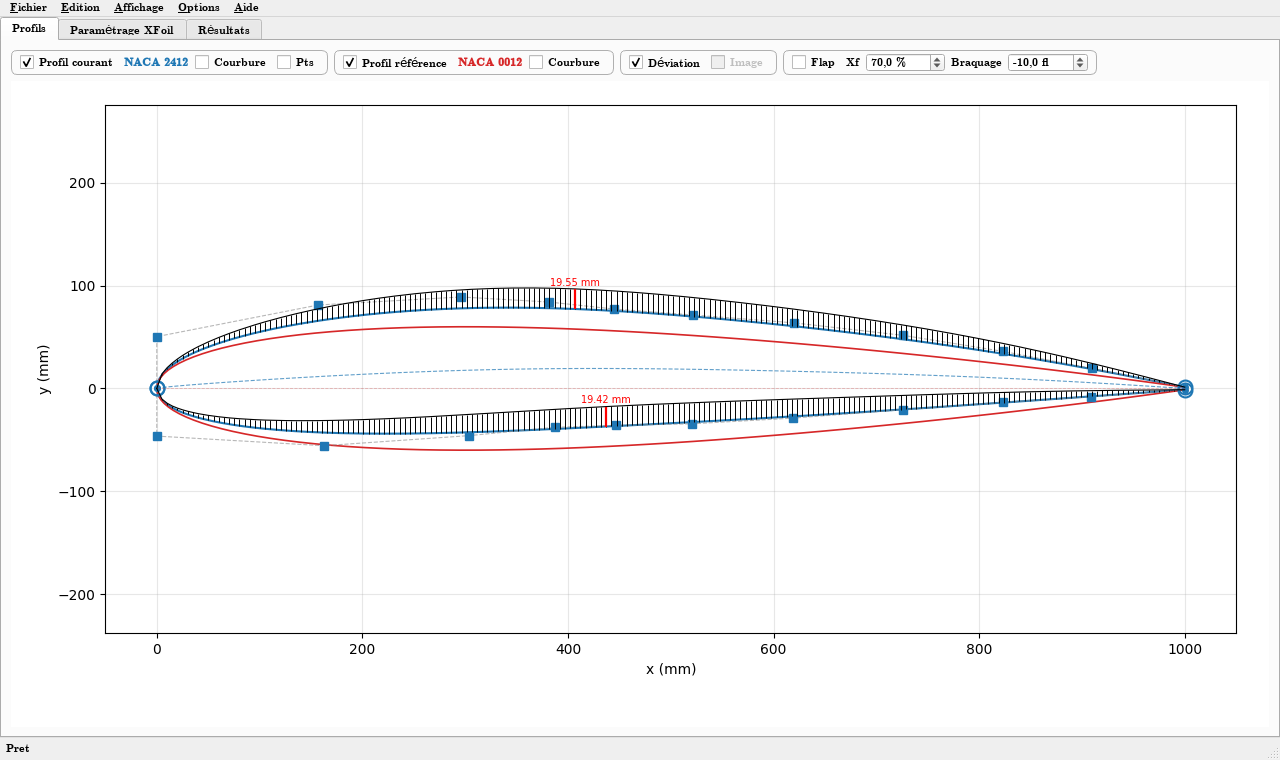
\includegraphics[width=0.49\textwidth]{images/06_tab_profils_deviation.png}}
    \hfill
    \fbox{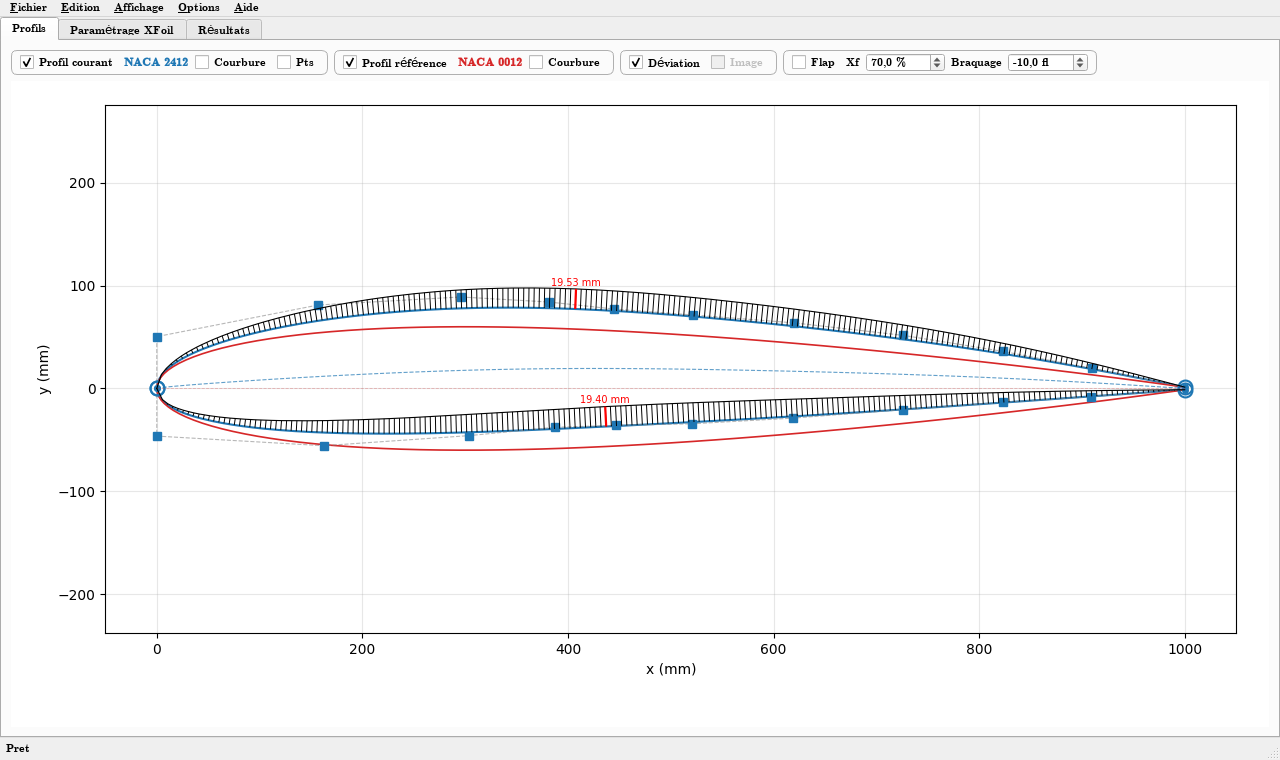
\includegraphics[width=0.49\textwidth]{images/14_deviation_normale.png}}
    \caption{Déviation entre NACA~2412 (courant, bleu) et NACA~0012
        (référence, rouge). À gauche le mode \emph{verticale}
        (quills verticaux), à droite le mode \emph{normale}
        (quills perpendiculaires à la surface). Dans les deux cas,
        le quill de déviation maximale est tracé en \textcolor{red}{rouge}
        avec sa valeur en millimètres.}
    \label{fig:06_tab_profils_deviation.png}
\end{figure}

\subsubsection*{Déviation maximale}

Le \textbf{maximum} de déviation est signalé par un quill
\textcolor{red}{\textbf{rouge}} portant sa \textbf{valeur en
millimètres} à son extrémité. Le calcul est effectué :

\begin{itemize}
    \item \textbf{par segment} de Bézier si le profil courant est en
        mode spline (un maximum par segment d'extrados et
        d'intrados) ;
    \item \textbf{par côté} (extrados, intrados) si le profil courant
        est en mode points discrets.
\end{itemize}

La valeur affichée est la déviation \textbf{réelle} (non
exagérée), exprimée dans l'unité du profil (millimètres pour une
corde de 1\,000~mm).

\begin{astuce}
Lorsque les profils ont une déviation très petite à l'œil
(par exemple lors d'une optimisation par petits déplacements
des points de contrôle), il est utile d'\textbf{amplifier}
l'affichage de la déviation. L'échelle est réglable via le
menu contextuel : \menu{Échelle déviation\dots}. Cette échelle
n'affecte que la longueur visuelle des quills, pas la valeur en
millimètres affichée au maximum.
\end{astuce}

\section{Charger un profil depuis la base UIUC}
\label{sec:uiuc}

AirfoilTools intègre un \textbf{accès direct} à la base de données
de profils de l'Université de l'Illinois (collection
\textbf{Selig}, environ 1\,600 profils), accessible via les entrées
\menu{Fichier $\rightarrow$ Depuis la base UIUC $\rightarrow$ Profil
courant\dots} et \menu{\dots Profil référence\dots}.

\screenshot{11_dialog_uiuc.png}{0.7}{%
    Dialogue de chargement depuis la base UIUC. La recherche
    \og naca \fg{} filtre 183~profils sur 1\,613. Le profil
    sélectionné affiche sa description sous la liste.}

\subsection{Utilisation}

\begin{enumerate}
    \item Au premier appel, l'index complet (~1\,600 profils) est
        téléchargé depuis le serveur UIUC. Le téléchargement prend
        quelques secondes selon la connexion.
    \item Saisir tout ou partie du nom ou de la description du
        profil dans le champ \menu{Recherche} : la liste se filtre
        en temps réel (insensible à la casse).
    \item Cliquer sur un profil pour voir sa description sous la
        liste. Double-clic ou bouton \bouton{Charger} pour le
        télécharger et l'ouvrir.
    \item Le profil est chargé en \textbf{mode points discrets}
        (format Selig). Pour bénéficier de l'édition interactive,
        utiliser ensuite \menu{Édition $\rightarrow$ Convertir en
        Spline} (voir section suivante).
\end{enumerate}

\subsection{Cache local}

Pour éviter de surcharger inutilement le serveur UIUC et pour
permettre l'utilisation hors ligne :

\begin{itemize}
    \item L'\textbf{index} (liste des profils + descriptions) est
        mis en cache pour \textbf{7~jours}. Au-delà, il est
        re-téléchargé automatiquement.
    \item Les \textbf{fichiers \chemin{.dat}} téléchargés sont mis
        en cache de manière \textbf{permanente} (les profils UIUC
        sont stables dans le temps).
\end{itemize}

Le bouton \bouton{Rafraichir} force le re-téléchargement de
l'index pour récupérer d'éventuels nouveaux profils.

L'emplacement du cache est :

\begin{itemize}
    \item Windows : \chemin{C:\textbackslash{}Users\textbackslash{}<utilisateur>\textbackslash{}.airfoiltools\textbackslash{}cache\textbackslash{}uiuc\textbackslash{}}
    \item Linux / macOS : \chemin{\textasciitilde/.airfoiltools/cache/uiuc/}
\end{itemize}

\begin{noteinfo}
Les fichiers \chemin{.dat} de la base UIUC suivent la
convention Selig (parcours BF $\rightarrow$ extrados $\rightarrow$
BA $\rightarrow$ intrados $\rightarrow$ BF) avec une ligne
d'en-tête contenant le nom du profil. Ils sont directement
exploitables par AirfoilTools.
\end{noteinfo}

\begin{attention}
Une connexion internet est requise pour le premier
téléchargement de l'index et de chaque profil. En cas
d'indisponibilité du serveur UIUC, le dialogue affiche un
message d'erreur ; les profils déjà mis en cache restent
toutefois utilisables.
\end{attention}

\section{Générer un profil NACA}
\label{sec:naca}

AirfoilTools sait générer à la volée les profils de la famille
\textbf{NACA} à partir de leur désignation, sans passer par un
fichier. La génération est accessible via \menu{Fichier
$\rightarrow$ Profil NACA $\rightarrow$ Profil courant\dots} (ou
\menu{\dots Profil référence\dots}).

\screenshot{16_dialog_naca.png}{0.55}{%
    Saisie des indices NACA. Un second dialogue demande ensuite le
    nombre de points du profil.}

\subsection{Utilisation}

\begin{enumerate}
    \item Saisir les \textbf{indices} dans le premier dialogue :
        \begin{itemize}
            \item \textbf{4 chiffres} (ex. \texttt{2412}) : cambrure
                maximale (\%), position de cambrure max (dixièmes de
                corde), épaisseur relative (\%) ;
            \item \textbf{5 chiffres} (ex. \texttt{23012}) : profil
                cambré à ligne moyenne plus complexe.
        \end{itemize}
    \item Saisir le \textbf{nombre de points} dans le second
        dialogue (par défaut 150).
    \item Le profil est généré, normalisé (corde 1\,000~mm) et
        affecté au rôle choisi (courant ou référence).
\end{enumerate}

\subsection{Régénération propre depuis le menu contextuel}

Un profil généré par cette fonction est \textbf{marqué} comme
profil NACA tant qu'il n'a pas été modifié (édition d'un point de
contrôle) ni converti en spline. Pour un tel profil NACA en mode
points discrets, le \textbf{menu contextuel} (clic droit) propose
l'entrée \menu{Nombre de points\dots}.

Changer le nombre de points par ce biais ne se contente pas
d'interpoler les points existants : il \textbf{rappelle la fonction
de génération NACA} pour produire un profil \emph{propre} à la
nouvelle résolution, conforme à la formule analytique.

\begin{noteinfo}
Cette régénération propre n'est possible que pour un profil NACA
\textbf{non modifié}. Dès qu'il est converti en spline ou édité,
le marqueur est perdu : on revient alors au ré-échantillonnage
classique de la spline.
\end{noteinfo}

\section{Conversion en spline}
\label{sec:convertspline}

Pour bénéficier de l'édition interactive, il faut convertir le
profil en mode spline. Cela se fait via :

\begin{itemize}
    \item le menu \menu{Édition $\rightarrow$ Convertir en Spline} ;
    \item le raccourci clavier \touche{Ctrl}+\touche{B}.
\end{itemize}

Un dialogue s'ouvre pour saisir les paramètres de conversion :

\screenshot{07_dialog_convert.png}{0.45}{%
    Dialogue de conversion en spline.}

\begin{tabularx}{\linewidth}{l X}
    \toprule
    \textbf{Paramètre} & \textbf{Description} \\
    \midrule
    Degré extrados
        & Degré des courbes de Bézier de l'extrados.
          Petit (3--5) = forme très lissée ; moyen (6--12) =
          compromis (recommandé) ; grand ($>$~15) = forme très
          précise mais risque d'oscillations.\\
    Degré intrados
        & Idem pour l'intrados. Peut être différent du degré
          extrados (typiquement intrados moins courbé).\\
    Tolérance
        & Déviation maximale acceptée entre la spline ajustée
          et les points discrets, en fraction de la corde.
          Valeur typique : $10^{-3}$ à $10^{-4}$.\\
    Max segments
        & Nombre maximal de segments de Bézier par côté.
          Avec 1, on obtient un seul segment global (comportement
          historique). Avec une valeur supérieure et une
          tolérance fine, l'algorithme \emph{adaptatif} découpe
          au point de plus grande erreur jusqu'à respecter la
          tolérance, concentrant les segments dans les zones de
          forte courbure (typiquement le bord d'attaque).\\
    Lissage
        & Coefficient de régularisation de l'ajustement
          (Tikhonov). $0$ = ajustement par moindres carrés pur ;
          $>0$ = lissage du polygone de contrôle.\\
    \bottomrule
\end{tabularx}

\begin{astuce}
Pour la plupart des profils, des paramètres de
\textbf{degré 11}, \textbf{tolérance $10^{-3}$},
\textbf{max segments 4}, \textbf{lissage 0{,}1} donnent un bon
compromis entre précision et qualité géométrique. Réduisez
la tolérance à $10^{-4}$ et augmentez \emph{Max segments} à
8--10 pour une approximation très fidèle.
\end{astuce}

\section{Édition interactive}

En mode spline, le canvas devient un \textbf{éditeur géométrique
interactif}.

\subsection{Interactions souris}

\begin{tabularx}{\linewidth}{l X}
    \toprule
    \textbf{Action} & \textbf{Effet} \\
    \midrule
    Clic gauche + déplacement sur un point de contrôle
        & Déplace le point de contrôle. La courbe est mise à
          jour en temps réel.\\
    Clic gauche + déplacement dans le vide
        & Trace un \emph{rectangle de zoom}. La vue est recadrée
          sur la zone à la fin du drag.\\
    Molette
        & Zoom centré sur la position du curseur.\\
    Clic milieu (ou \touche{Maj}+clic gauche)
        & Pan (translation de la vue).\\
    Clic droit
        & Ouvre le \textbf{menu contextuel}.\\
    \bottomrule
\end{tabularx}

\subsection{Menu contextuel (clic droit)}

Le menu contextuel offre plusieurs actions selon le contexte :

\begin{itemize}
    \item \menu{Info point\dots} (si clic sur un point de contrôle) :
        affiche les coordonnées et les paramètres locaux du point.
    \item \menu{Libérer la contrainte de tangence verticale au bord
        d'attaque} (si clic sur le nœud P1, voisin du bord d'attaque) :
        libère ou rétablit la tangente verticale au bord d'attaque.
        Voir la section~\ref{sec:batangente}.
    \item \menu{Échelle porcupines\dots} : règle l'échelle
        d'affichage de la courbure.
    \item \menu{Densité porcupines / $\times 2$ ou $\div 2$} :
        modifie le nombre de quills affichés.
    \item \menu{Échelle déviation\dots} et \menu{Densité déviation} :
        idem pour les porcupines de déviation.
    \item \menu{Split extrados / Split intrados} (en mode spline) :
        scinde la spline en deux au point cliqué le plus proche
        (algorithme de De Casteljau, exact).
    \item \menu{Paramètres globaux} : nombre de points
        d'échantillonnage, méthode (curviligne ou adaptative).
    \item \menu{Segment} (si clic dans un segment précis) :
        permet de définir des \emph{overrides per-segment}
        (degré, nombre de points, méthode différente du global).
\end{itemize}

\subsection{Tangente verticale au bord d'attaque}
\label{sec:batangente}

Par défaut, le premier point de contrôle intérieur de chaque côté
(noté \textbf{P1}, voisin du bord d'attaque) est \textbf{contraint}
à rester sur la verticale du bord d'attaque (BA). Cette contrainte
garantit une \textbf{tangente verticale} au bord d'attaque, ce qui
correspond à la géométrie naturelle de la plupart des profils. Lors
de l'édition, le déplacement de P1 est donc limité à l'axe vertical.

\screenshot{13_ba_tangente.png}{1.0}{%
    Effet de la contrainte de tangente verticale au bord d'attaque.
    À gauche, contrainte active : le nœud P1 (entouré en rouge) reste
    aligné verticalement avec le BA, la tangente (pointillé rouge) est
    verticale. À droite, contrainte libérée : P1 peut être déplacé
    librement, la tangente s'incline.}

Il est parfois souhaitable de \textbf{libérer} cette contrainte (par
exemple pour décalquer un profil dont le bord d'attaque n'a pas une
tangente strictement verticale). Pour cela :

\begin{enumerate}
    \item Effectuer un \textbf{clic droit} sur le nœud P1 de
        l'extrados ou de l'intrados.
    \item Choisir \menu{Libérer la contrainte de tangence verticale
        au bord d'attaque}.
\end{enumerate}

Le nœud P1 devient alors librement déplaçable (en $x$ et en $y$).
Pour rétablir la contrainte, refaire un clic droit sur le nœud et
choisir \menu{Rétablir la tangence verticale au bord d'attaque} :
le nœud P1 est automatiquement ramené sur la verticale du bord
d'attaque.

\begin{noteinfo}
La contrainte est gérée \textbf{indépendamment} pour l'extrados et
l'intrados. Libérer la tangente côté extrados n'affecte pas
l'intrados, et inversement.
\end{noteinfo}

\section{Volet (flap)}
\label{sec:flap}

Le module \textbf{volet} génère un \textbf{profil braqué} à partir
du profil courant, en faisant pivoter sa partie arrière autour d'un
axe d'articulation. Le profil avec volet est tracé en
\textbf{vert}, en plus du courant et de la référence ; il est
\textbf{non modifiable} (recalculé automatiquement) et peut être
simulé puis sauvegardé comme le profil courant.

\screenshot{15_tab_profils_flap.png}{1.0}{%
    Profil avec volet (vert) braqué à $-10^\circ$ à 70~\% de corde,
    superposé au profil courant (bleu) et à ses points de contrôle.}

\subsection{Activation et réglages}

Les contrôles se trouvent dans le cadre \og Flap \fg{} de la barre
de l'onglet \menu{Profils} :

\begin{tabularx}{\linewidth}{l X}
    \toprule
    \textbf{Contrôle} & \textbf{Rôle} \\
    \midrule
    \textbf{Flap} & Active la génération du profil braqué (vert). \\
    \textbf{Xf} & Position de l'axe d'articulation, en \textbf{pourcent
        de corde} mesuré depuis le bord d'attaque (5 à 95~\%). \\
    \textbf{Braquage} & Angle de braquage en degrés ($-45$ à
        $+45$). \textbf{Positif} = bord de fuite vers le \textbf{haut} ;
        \textbf{négatif} = bord de fuite vers le \textbf{bas}. \\
    \bottomrule
\end{tabularx}

Le profil braqué est recalculé en temps réel à chaque changement
de \menu{Xf} ou de \menu{Braquage}, et à chaque modification du
profil courant.

\subsection{Géométrie de l'articulation}

L'axe d'articulation est le \textbf{centre du cercle inscrit}
tangent simultanément à l'extrados et à l'intrados, dont l'abscisse
vaut \menu{Xf}. La partie arrière de chaque surface est ensuite
tournée de l'angle de braquage autour de cet axe.

\screenshot{19_flap_schema.png}{0.95}{%
    Construction de l'articulation : le cercle inscrit (vert),
    tangent à l'extrados et à l'intrados à l'abscisse $X_f$, fournit
    le centre de rotation (point rouge) du volet.}

Selon le côté et le signe du braquage, le raccord entre la partie
fixe et la partie braquée est traité différemment :

\begin{itemize}
    \item du côté où le braquage \textbf{ouvre} un jeu, un
        \textbf{arc de cercle} comble l'espace ;
    \item du côté où le braquage \textbf{referme} la matière, la
        surface est \textbf{coupée à l'intersection} (recouvrement
        retiré).
\end{itemize}

\subsection{Simulation et sauvegarde}

\begin{itemize}
    \item \textbf{Simulation} : le profil avec volet est simulé par
        XFoil au même titre que le courant et la référence. Le bouton
        \bouton{Flap seul} de l'onglet \menu{Paramétrage XFoil} le
        calcule isolément ; \bouton{Lancer tout} l'inclut s'il est
        actif. Les résultats apparaissent sous le rôle
        \emph{Volet} (vert) dans l'onglet \menu{Résultats}.
    \item \textbf{Sauvegarde} : \menu{Fichier $\rightarrow$
        Sauvegarder profil avec volet\dots} enregistre le profil
        braqué, avec le même choix complet / extrados / intrados et
        les mêmes formats que le profil courant.
\end{itemize}

\begin{important}
Pour la simulation, le profil avec volet est exprimé dans le
\textbf{repère normalisé du profil courant} : XFoil ne le
renormalise ni ne le redresse. On observe ainsi uniquement
l'effet du braquage par rapport au profil courant (déplacement de
la polaire, du moment, etc.), sans artefact de changement de corde
ou d'incidence de référence.
\end{important}

\section{Image de calque (décalquer un profil)}
\label{sec:calque}

AirfoilTools permet de charger une \textbf{image en arrière-plan}
(photo, scan d'un plan, capture d'écran d'un profil) afin de
\textbf{décalquer} sa forme en déplaçant les points de contrôle du
profil courant jusqu'à épouser la silhouette de l'image.

\screenshot{12_tab_profils_calque.png}{1.0}{%
    Décalquage d'un profil : l'image de calque (silhouette grise) est
    affichée en arrière-plan ; le profil courant (bleu, en mode spline)
    et ses points de contrôle se superposent par-dessus. On ajuste les
    points de contrôle pour faire coïncider la courbe bleue avec la
    silhouette.}

\subsection{Chargement de l'image}

Le chargement se fait via \menu{Fichier $\rightarrow$ Charger image
de calque\dots}. Les formats usuels sont acceptés : \chemin{.jpg},
\chemin{.png}, \chemin{.tif}, \chemin{.bmp}. À l'ouverture, l'image
est mise à l'échelle pour couvrir approximativement la corde
(1\,000~mm) et la case \textbf{Image} de la barre de contrôle
devient active et cochée.

L'image est dessinée \textbf{en arrière-plan}, sous le profil et ses
points de contrôle, qui restent donc parfaitement visibles et
manipulables par-dessus.

\subsection{Positionner, mettre à l'échelle et tourner l'image}

Les manipulations de l'image se font en maintenant la touche
\touche{i} enfoncée, combinée à la souris :

\begin{tabularx}{\linewidth}{l X}
    \toprule
    \textbf{Action} & \textbf{Effet} \\
    \midrule
    \touche{i} + clic gauche glissé
        & \textbf{Déplace} l'image (translation).\\
    \touche{i} + molette
        & \textbf{Met à l'échelle} l'image (agrandit / réduit autour
          de son centre).\\
    \touche{i} + clic droit glissé
        & \textbf{Tourne} l'image autour de l'origine $(0,0)$
          (le bord d'attaque).\\
    \touche{Maj} + \touche{i} + action
        & \textbf{Ajustements fins} : déplacement et rotation
          dix fois plus lents, pas d'échelle réduit. Idéal pour le
          calage précis.\\
    \bottomrule
\end{tabularx}

\begin{astuce}
Procédez en deux temps : d'abord un calage grossier (déplacement,
échelle, rotation sans \touche{Maj}) pour superposer
approximativement l'image et le profil, puis un \textbf{ajustement
fin} en maintenant \touche{Maj} pour le calage précis du bord
d'attaque et du bord de fuite.
\end{astuce}

\begin{noteinfo}
Le canvas doit avoir le \textbf{focus clavier} pour que la touche
\touche{i} soit prise en compte : il l'obtient automatiquement
dès que le curseur survole la zone de tracé.
\end{noteinfo}

\subsection{Masquer ou retirer l'image}

\begin{itemize}
    \item La case \textbf{Image} de la barre de contrôle affiche ou
        masque l'image sans la supprimer.
    \item \menu{Fichier $\rightarrow$ Retirer l'image de calque}
        supprime définitivement l'image de la session.
\end{itemize}

\begin{important}
L'image de calque et sa position (échelle, rotation, translation)
sont \textbf{enregistrées avec le projet} au format \chemin{.aftproj}
(voir chapitre~\ref{chap:formats}). On retrouve ainsi son calque
exactement tel qu'il était à la réouverture du projet. Les formats
de profil classiques (\chemin{.dat}, \chemin{.bspl}\dots) ne
contiennent \textbf{pas} l'image : pour conserver le calque, il faut
enregistrer un projet.
\end{important}

\section{Avertissement \og Courbure indisponible \fg{}}

Lorsque la case \menu{Courbure} est activée alors que le profil
concerné est en mode points discrets (non converti en spline),
un message d'information s'affiche :

\screenshot{08_msg_courbure.png}{0.7}{%
    Message d'avertissement \og Courbure indisponible \fg{}.}

Comme indiqué dans le message, deux solutions sont possibles :

\begin{enumerate}
    \item convertir le profil en spline (menu
        \menu{Édition $\rightarrow$ Convertir en Spline}) ;
    \item charger un profil dans un format préservant la
        géométrie spline (\chemin{.bspl} ou \chemin{.bez}).
\end{enumerate}

La case se décoche automatiquement après affichage du message.

\section{Modification du nombre de points}

En mode spline, le nombre de points d'échantillonnage discret
des splines est modifiable via le menu \menu{Édition $\rightarrow$
Échantillonnage $\rightarrow$ Profil courant\dots} (ou
\menu{\dots Profil référence\dots}).

Un dialogue demande le nouveau nombre de points (entre 10 et
10\,000). Cela affecte uniquement la \emph{discrétisation
d'export} et l'affichage : la géométrie spline sous-jacente
n'est pas altérée.

\begin{noteinfo}
Pour les simulations XFoil, l'échantillonnage par défaut
(150~points) est généralement suffisant. XFoil ré-échantillonne
ensuite en interne via la commande \texttt{PANE} si l'option
\emph{Repanel} est activée dans l'onglet \menu{Paramétrage XFoil}.
\end{noteinfo}
